\documentclass{standalone}

%----- Pacchetti ---------------------------------------------
\usepackage{amsmath}         
\usepackage{mathtools}       
\usepackage{amssymb}   
\usepackage{amsthm}         
\usepackage{tikz}
\usepackage{tikz-cd}
\usepackage{tikz-3dplot}
\usepackage{graphicx}
\usepackage{thmtools}
\usepackage[all]{xy}        
\usetikzlibrary{decorations.markings, arrows.meta}
\usetikzlibrary{hobby}
\usepackage{pgfplots}
\pgfplotsset{compat=1.18}
\usepackage[absolute ,overlay]{textpos}
\usepackage[dvipsnames]{xcolor}

\begin{document}
	
	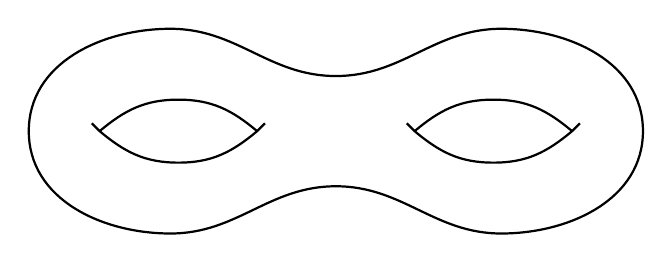
\begin{tikzpicture}
%	\draw[help lines] (-4,-2)grid(4,2);
	
	\draw[thick] (-3.9,0) to[out=90, in=180](-2.1,1.3)to[out=0, in=180](0,.7)to[out=0,in=180](2.1,1.3) to[out=0, in=90](3.9,0);

	\draw[thick] (-3.9,0) to[out=270, in=180](-2.1,-1.3)to[out=0, in=180](0,-.7)to[out=0,in=180](2.1,-1.3) to[out=0, in=270](3.9,0);
	
	%buchi
	\draw[thick](-3.1,.1)to (-3,0) to[out=320,in=180] (-2,-.4) to [out=0, in=220](-1,0)to (-.9,.1);
	\draw[thick](-3,0) to[out=40,in=180] (-2,.4) to [out=0, in=140](-1,0);
	
	
	\draw[thick](.9,.1)to (1,0) to[out=320,in=180] (2,-.4) to [out=0, in=220](3,0)to (3.1,.1);
	\draw[thick](1,0) to[out=40,in=180] (2,.4) to [out=0, in=140](3,0);
	
	
	\end{tikzpicture}
	
\end{document}